\documentclass[12pt]{report}
\usepackage[utf8]{inputenc}
\usepackage[russian]{babel}
%\usepackage[14pt]{extsizes}
\usepackage{listings}
\usepackage{graphicx}
\usepackage{amsmath,amsfonts,amssymb,amsthm,mathtools} 
\usepackage{pgfplots}
\usepackage{filecontents}
\usepackage{indentfirst}
\usepackage{eucal}
\usepackage{enumitem}
\frenchspacing

\usepackage{indentfirst} % Красная строка


\usetikzlibrary{datavisualization}
\usetikzlibrary{datavisualization.formats.functions}

\usepackage{amsmath}




% Для листинга кода:
\lstset{ %
	language=python,                 % выбор языка для подсветки
	basicstyle=\small\sffamily, % размер и начертание шрифта для подсветки кода
	keywordstyle=\color{blue},
	numbers=left,               % где поставить нумерацию строк (слева\справа)
	numberstyle=\tiny,           % размер шрифта для номеров строк
	stepnumber=1,                   % размер шага между двумя номерами строк
	numbersep=5pt,                % как далеко отстоят номера строк от подсвечиваемого кода
	showspaces=false,            % показывать или нет пробелы специальными отступами
	showstringspaces=false,      % показывать или нет пробелы в строках
	showtabs=false,             % показывать или нет табуляцию в строках
	frame=single,              % рисовать рамку вокруг кода
	tabsize=2,                 % размер табуляции по умолчанию равен 2 пробелам
	captionpos=t,              % позиция заголовка вверху [t] или внизу [b] 
	breaklines=true,           % автоматически переносить строки (да\нет)
	breakatwhitespace=false, % переносить строки только если есть пробел
	escapeinside={\#*}{*)}   % если нужно добавить комментарии в коде
}

\usepackage[left=2cm,right=2cm, top=2cm,bottom=2cm,bindingoffset=0cm]{geometry}
% Для измененных титулов глав:
\usepackage{titlesec, blindtext, color} % подключаем нужные пакеты
\definecolor{gray75}{gray}{0.75} % определяем цвет
\newcommand{\hsp}{\hspace{20pt}} % длина линии в 20pt
% titleformat определяет стиль
\titleformat{\chapter}[hang]{\Huge\bfseries}{\thechapter\hsp\textcolor{gray75}{|}\hsp}{0pt}{\Huge\bfseries}


% plot
\usepackage{pgfplots}
\usepackage{filecontents}
\usetikzlibrary{datavisualization}
\usetikzlibrary{datavisualization.formats.functions}

\begin{document}
	\def\contentsname{Содержание}
	\def\refname{Список литературы}
	\thispagestyle{empty}
	\begin{titlepage}
		\noindent \begin{minipage}{0.15\textwidth}
			
\includegraphics[width=\linewidth]{b_logo}
		\end{minipage}
		\noindent\begin{minipage}{0.9\textwidth}\centering
			\textbf{Министерство науки и высшего образования Российской Федерации}\\
			\textbf{Федеральное государственное бюджетное образовательное учреждение высшего образования}\\
			\textbf{~~~«Московский государственный технический университет имени Н.Э.~Баумана}\\
			\textbf{(национальный исследовательский университет)»}\\
			\textbf{(МГТУ им. Н.Э.~Баумана)}
		\end{minipage}
		
		\noindent\rule{18cm}{3pt}
		\newline\newline
		\noindent ФАКУЛЬТЕТ $\underline{\text{«Информатика и системы управления»}}$ \newline\newline
		\noindent КАФЕДРА $\underline{\text{«Программное обеспечение ЭВМ и информационные технологии»}}$\newline\newline\newline\newline\newline
		
		
		\begin{center}
			\noindent\begin{minipage}{1.3\textwidth}\centering
				\Large\textbf{  Отчет по лабораторной работе №1}\newline
				\textbf{по дисциплине "Анализ алгоритмов"}\newline\newline
			\end{minipage}
		\end{center}
		
		\noindent\textbf{Тема} $\underline{\text{Расстояние Левенштейна и Дамерау-Левенштейна}}$\newline\newline
		\noindent\textbf{Студент} $\underline{\text{Петрова А.А.}}$\newline\newline
		\noindent\textbf{Группа} $\underline{\text{ИУ7-56Б}}$\newline\newline
		\noindent\textbf{Оценка (баллы)} $\underline{\text{~~~~~~~~~~~~~~~~~~~~~~~~~~~}}$\newline\newline
		\noindent\textbf{Преподаватели} $\underline{\text{Волкова Л.Л.}}$\newline\newline\newline
		
		\begin{center}
			\vfill
			Москва~---~\the\year
			~г.
		\end{center}
	\end{titlepage}
	
	
	\tableofcontents
	
	\newpage
	\chapter*{Введение}
	\addcontentsline{toc}{chapter}{Введение}
	\textbf{Расстояние Левенштейна} - минимальное количество операций вставки одного символа, удаления одного символа и замены одного символа на другой, необходимых для превращения одной строки в другую.
	\newline
	
	Расстояние Левенштейна применяется в теории информации и компьютерной лингвистики для:
	
	\begin{itemize}
		\item исправления ошибок в слове;
		\item сравнения текстовых файлов утилитой diff;
		\item в биоинформатике для сравнения генов, хромосом и белков.
	\end{itemize}
	
	Целью работы является реализация и оценка алгоритмов нахождения расстояния Левенштейна и Дамерау-Левенштейна.
	
	Для достижения поставленной цели необходимо выполнить следующие задачи:
	
	\begin{itemize}
		\item изучить алгоритмы Левенштейна и Дамерау-Левенштейна (аналитическая часть);
		\item создать схемы указанных алгоритмов (матричных и рекусривных) (конструкторская часть);
		\item реализовать эти алгоритмы (технологическая часть);
		\item провести анализ линейной и рекурсивной реализаций выбранного алгоритма определения расстояния между строками по затрачиваемым ресурсам (времени и памяти) (исследовательская часть);
		\item описать и обосновать полученные результаты в отчете о выполненной лабораторной работе, выполненного как расчётно-пояснительная записка к работе.
	\end{itemize}
	
	\chapter{Аналитическая часть}
	
	Расстояние Левенштейна \cite{Levenshtein} между двумя строками — это минимальное количество операций вставки, удаления и замены, необходимых для превращения одной строки в другую.
	
	
	Цены операций могут зависеть от вида операции (вставка (insert), удаление (delete), замена (replace) и/или от участвующих в ней символов, отражая разную вероятность разных ошибок при вводе текста, и т. п. В общем случае:
	
	\begin{itemize}
		\item $w(a,b)$ — цена замены символа $a$ на символ $b$.
		\item $w(\lambda,b)$ — цена вставки символа $b$.
		\item $w(a,\lambda)$ — цена удаления символа $a$.
	\end{itemize}
	
	Для решения задачи о редакционном расстоянии необходимо найти последовательность замен, минимизирующую суммарную цену. Расстояние Левенштейна является частным случаем этой задачи при
	
	\begin{itemize}
		\item $w(a,a)=0$.
		\item $w(a,b)=1, \medspace a \neq b$.
		\item $w(\lambda,b)=1$.
		\item $w(a,\lambda)=1$.
	\end{itemize}
	
	\section{Рекурсивный алгоритм нахождения расстояния Левенштейна}
	
	Расстояние Левенштейна между двумя строками a и b может быть вычислено по формуле \ref{eq:D}, где $|a|$ означает длину строки $a$; $a[i]$ — i-ый символ строки $a$ , функция $D(i, j)$ определена как:
	\begin{equation}
		\label{eq:D}
		D(i, j) = \begin{cases}
			0 &\text{i = 0, j = 0}\\
			i &\text{j = 0, i > 0}\\
			j &\text{i = 0, j > 0}\\
			\min \lbrace \\
			\qquad D(i, j-1) + 1\\
			\qquad D(i-1, j) + 1 &\text{i > 0, j > 0}\\
			\qquad D(i-1, j-1) + m(a[i], b[j]) &\text(\ref{eq:m})\\
			\rbrace
		\end{cases},
	\end{equation}
	
	а функция \ref{eq:m} определена как:
	\begin{equation}
		\label{eq:m}
		m(a, b) = \begin{cases}
			0 &\text{если a = b,}\\
			1 &\text{иначе}
		\end{cases}.
	\end{equation}
	
	
	Рекурсивный алгоритм реализует формулу \ref{eq:D}.
	Функция $D$ составлена из следующих соображений:
	\begin{enumerate}
		\item Для перевода из пустой строки в пустую требуется ноль операций;
		\item Для перевода из пустой строки в строку $a$ требуется $|a|$ операций;
		\item Для перевода из строки $a$ в пустую требуется $|a|$ операций;
		\item Для перевода из строки $a$ в строку $b$ требуется выполнить последовательно некоторое количество операций (удаление, вставка, замена) в некоторой последовательности. Последовательность проведения любых двух операций можно поменять, порядок проведения операций не имеет никакого значения. Полагая, что $a', b'$  — строки $a$ и $b$ без последнего символа соответственно, цена преобразования из строки $a$ в строку $b$ может быть выражена как:
		\begin{enumerate}
			\item Сумма цены преобразования строки $a$ в $b$ и цены проведения операции удаления, которая необходима для преобразования $a'$ в $a$;
			\item Сумма цены преобразования строки $a$ в $b$  и цены проведения операции вставки, которая необходима для преобразования $b'$ в $b$;
			\item Сумма цены преобразования из $a'$ в $b'$ и операции замены, предполагая, что $a$ и $b$ оканчиваются разные символы;
			\item Цена преобразования из $a'$ в $b'$, предполагая, что $a$ и $b$ оканчиваются на один и тот же символ.
		\end{enumerate}
		Минимальной ценой преобразования будет минимальное
		значение приведенных вариантов.
	\end{enumerate}
	
	\section{Матричный алгоритм нахождения расстояния Левенштейна}
	
	Прямая реализация формулы \ref{eq:D} может быть малоэффективна по времени исполнения при больших $i, j$, т. к. множество промежуточных значений $D(i, j)$ вычисляются заново множество раз подряд. Для оптимизации нахождения расстояния Левенштейна можно использовать матрицу в целях хранения соответствующих промежуточных значений. В таком случае алгоритм представляет собой построчное заполнение матрицы
	
	$A_{|a|,|b|}$ значениями $D(i, j)$.
	
	
	\section{Рекурсивный алгоритм нахождения расстояния Левенштейна с заполнением матрицы}
	
	\label{sec:recmat}
	
	
	Рекурсивный алгоритм заполнения можно оптимизировать по времени выполнения с использованием матричного алгоритма. Суть данного метода заключается в параллельном заполнении матрицы при выполнении рекурсии. В случае, если рекурсивный алгоритм выполняет прогон для данных, которые еще не были обработаны, результат нахождения расстояния заносится в матрицу. В случае, если обработанные ранее данные встречаются снова, для них расстояние не находится и алгоритм переходит к следующему шагу.
	
	
	\section{Расстояния Дамерау — Левенштейна}
	
	Расстояние Дамерау — Левенштейна \cite{Damerau} может быть найдено по формуле \ref{eq:d}, которая задана как
	
	\begin{equation}
		\label{eq:d}
		d_{a,b}(i, j) = \begin{cases}
			\max(i, j), &\text{если }\min(i, j) = 0,\\
			\min \lbrace \\
			\qquad d_{a,b}(i, j-1) + 1,\\
			\qquad d_{a,b}(i-1, j) + 1,\\
			\qquad d_{a,b}(i-1, j-1) + m(a[i], b[j]), &\text{иначе}\\
			\qquad \left[ \begin{array}{cc}d_{a,b}(i-2, j-2) + 1, &\text{если }i,j > 1;\\
				\qquad &\text{}a[i] = b[j-1]; \\
				\qquad &\text{}b[j] = a[i-1]\\
				\qquad \infty, & \text{иначе}\end{array}\right.\\
			\rbrace
		\end{cases},
	\end{equation}
	
	Формула выводится по тем же соображениям, что и формула (\ref{eq:D}).
	Как и в случае с рекурсивным методом, прямое применение этой формулы неэффективно по времени исполнения, то аналогично методу из \ref{sec:recmat} производится добавление матрицы для хранения промежуточных значений рекурсивной формулы.
	
	\section{Вывод}
	В данном разделе были рассмотрены алгоритмы нахождения расстояния Левенштейна и Дамерау-Левенштейна, который является модификаций первого, учитывающего возможность перестановки соседних символов. Формулы Левенштейна и Дамерау — Левенштейна для рассчета расстояния между строками задаются рекурсивно, а следовательно, алгоритмы могут быть реализованы рекурсивно или итерационно.
	
	\clearpage
	
	\chapter{Конструкторская часть}
	
	\section{Схемы алгоритмов}
	В данной части будут рассмотрены схемы алгоритмов нахождения расстояние Левештейна и Дамерау - Левенштейна. На рисунках 2.1 - 2.4 представлены рассматриваемые алгоритмы.
	
	\begin{figure}[h]
		\centering
		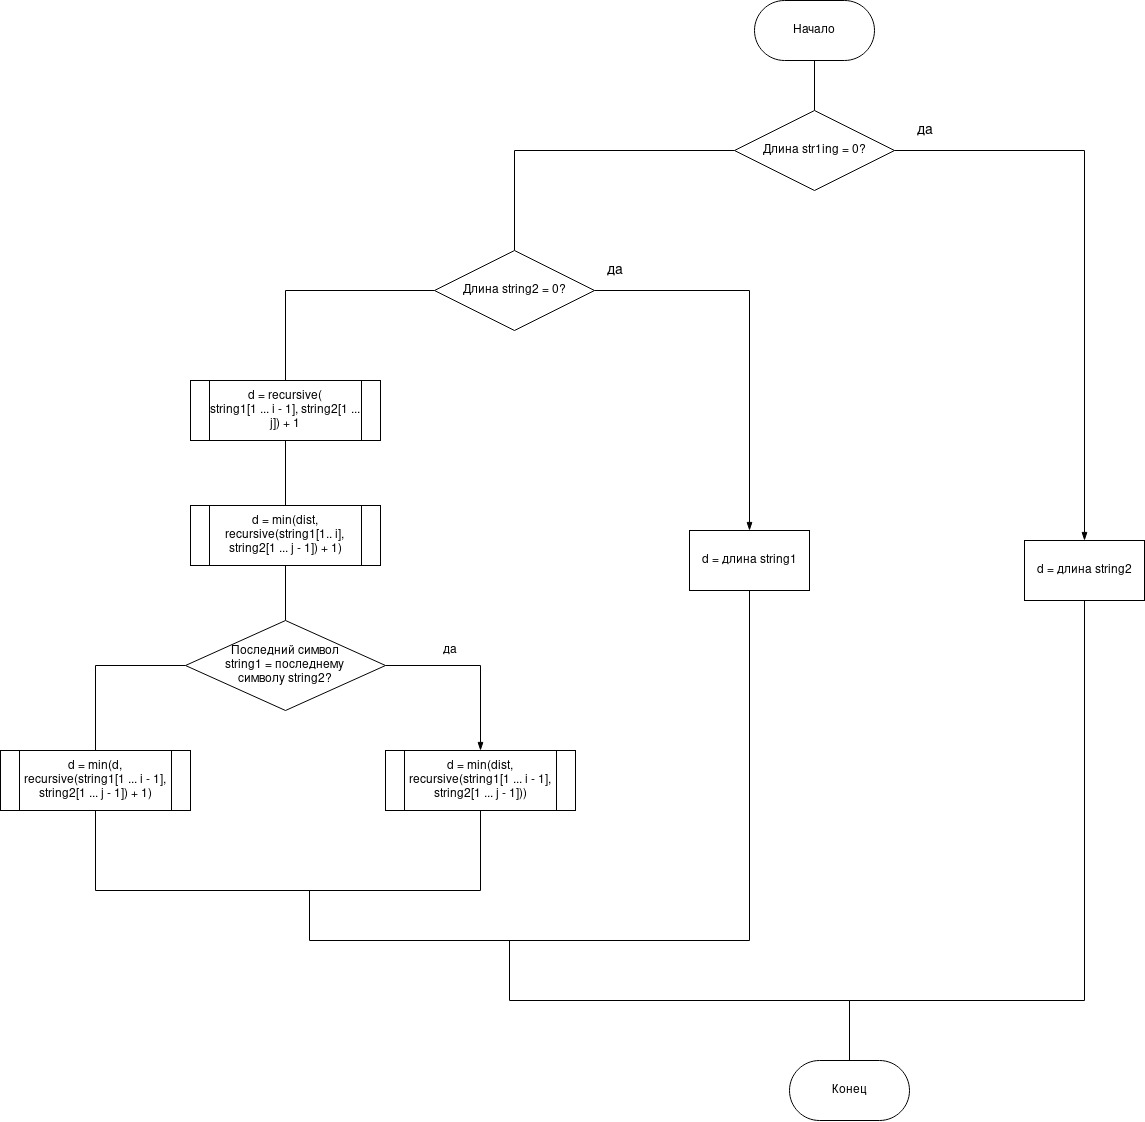
\includegraphics[width=0.75\linewidth]{rec.jpg}
		\caption{Схема рекурсивного алгоритма нахождения расстояния Левенштейна}
		\label{fig:mpr}
	\end{figure}
	
	\begin{figure}[h]
		\centering
		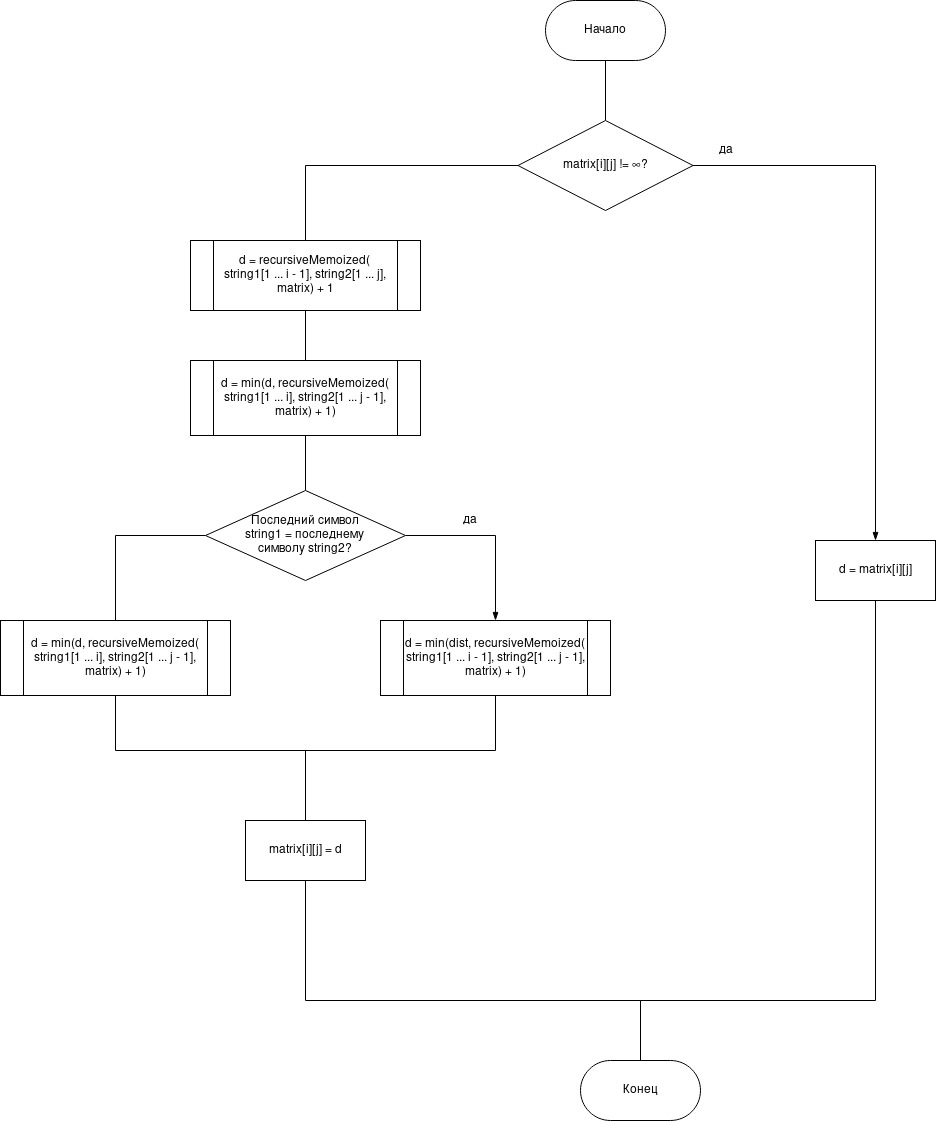
\includegraphics[scale=0.35]{mem.jpg}
		\caption{Схема рекурсивного алгоритма Левенштейна с кэшем}
		\label{fig:mpr}
	\end{figure}

	\begin{figure}[h]
		\centering
		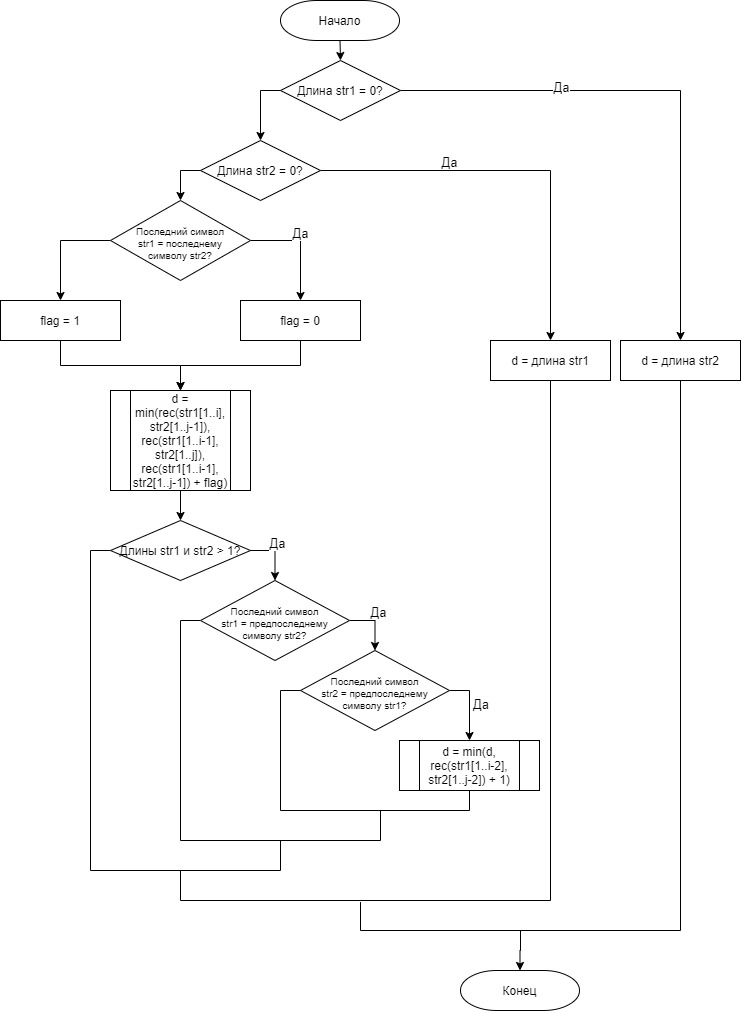
\includegraphics[scale=0.6]{rec_dl.jpg}
		\caption{Схема рекурсивного алгоритма нахождения расстояния Дамерау-Левенштейна}
		\label{fig:mpr}
	\end{figure}
	
	\begin{figure}[h]
		\centering
		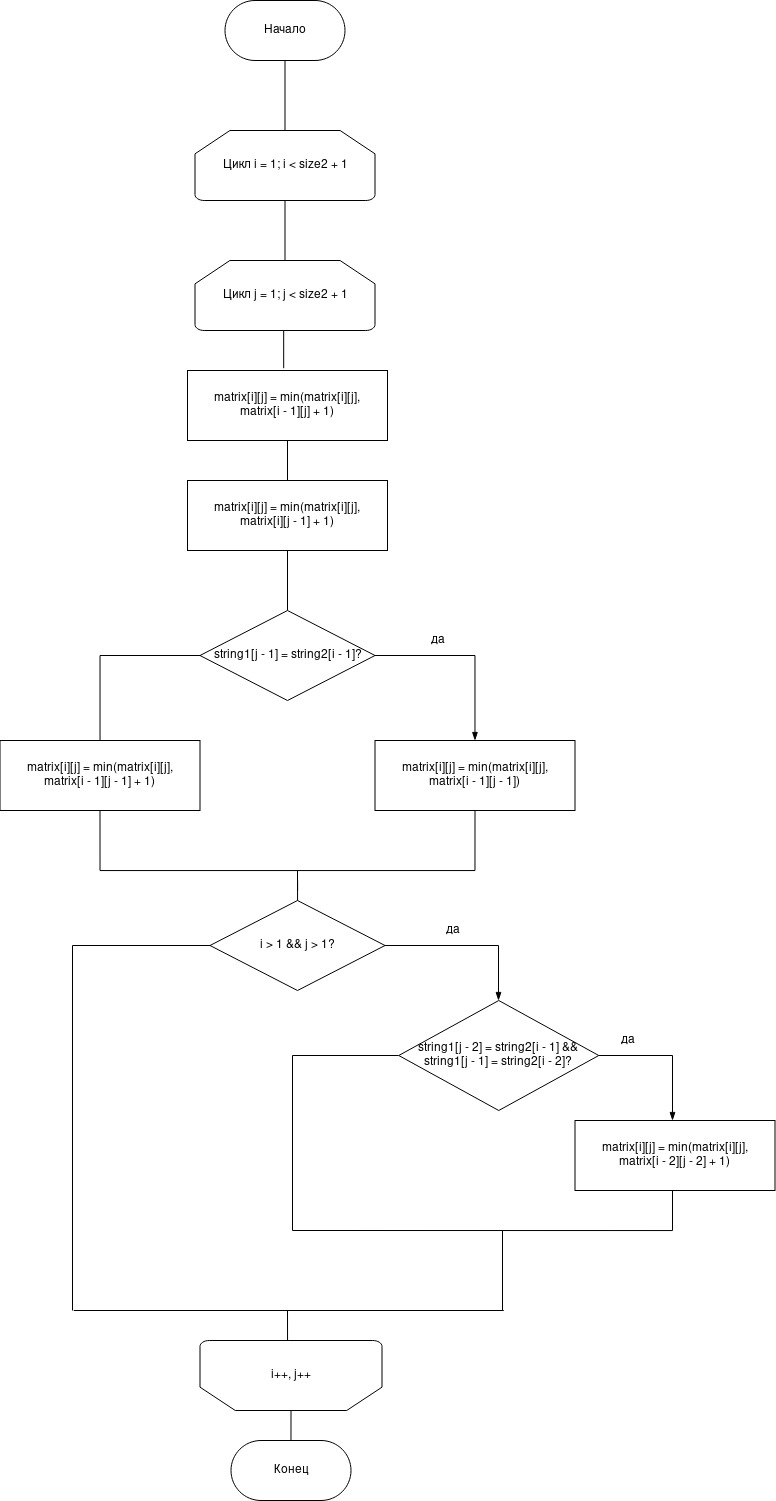
\includegraphics[scale=0.4]{iter_dl.jpg}
		\caption{Схема итеративного алгоритма нахождения расстояния Дамерау-Левенштейна}
		\label{fig:mpr}
	\end{figure}
	
	\section{Вывод}
	На основе теоретических данных, полученные в аналитическом разделе были построены схемы иследуеммых  алгоритмов.
	
	\chapter{Технологическая часть}
	
	\section{Требования к ПО}
	\textbf{Требования к вводу:}
	\begin{itemize}
		\item на вход подаются две строки в любой раскладке (в том числе и пустые);
		\item ПО должно выводить полученное расстояние и использованные матрицы;
		\item ПО должно выводить потраченное время.
	\end{itemize}
	\textbf{Требования к самому ПО:}
	\begin{itemize}
		\item ПО должно содержать 2 раздела: пользовательский (ручной ввод) и экспериментальный (для замеров времени);
		\item в пользовательском разделе должна присутствовать проверка на некорректные данные;
		\item пустая строка в поле для ввода строки должна считаться корректным данным.
	\end{itemize}
	
	\section{Средства реализации}
	Для реализации программы нахождения расстояния Левенштейна был выбран язык программирования Python. Данный выбор обусловлен тем, что этот язык наиболее удобен для работы со строками, а также тем, что в нём присутсвует функция для измерения процессорного времени.
	
	\section{Реализация алгоритмов}
	
	В листингах 3.1 - 3.4 приведена реализация алгоритмов нахождения расстояния Левенштейна и Дамерау-Левенштейна.
	
	\begin{lstlisting}[label=some-code,caption=Функция нахождения расстояния Левенштейна рекурсивно,language=Python]
	def lev_recursion(str1, str2, len1, len2):
		if (len1 == len2) and len1 == 0:
			return 0
		elif len1 == 0:
			return len2
		elif len2 == 0:
			return len1
		else:
			flag = bool(not (str1[len1 - 1] == str2[len2 - 1]))
		return min(min(lev_recursion(str1, str2, len1 - 1, len2) + 1,
					   lev_recursion(str1, str2, len1, len2 - 1) + 1),
					   lev_recursion(str1, str2, len1 - 1, len2 - 1) + flag)
	\end{lstlisting}
	
	\begin{lstlisting}[label=some-code,caption=Функция нахождения расстояние Левенштейна рекурсивно с помощью кэша,language=Python]
	def lev_cache(str1, str2, len1, len2, mtx):
		if not mtx[len1][len2] == 0:
			return mtx[len1][len2]
		elif (len1 == len2) and (len1 == 0):
			mtx[len1][len2] = 0
		elif len1 == 0:
			mtx[len1][len2] = len2
		elif len2 == 0:
			mtx[len1][len2] = len1
		else:
			flag = bool(not(str1[len1 - 1] == str2[len2 - 1]))
			mtx[len1][len2] = min(min(lev_cache(str1, str2, len1 - 1, len2, mtx) + 1,
									  lev_cache(str1, str2, len1, len2 - 1, mtx) + 1),
									  lev_cache(str1, str2,  len1 - 1, len2 - 1, mtx) + flag)
		return mtx[len1][len2]
		
	def rec_lev_cache(str1, str2, len1, len2):
		mtx = [[0 for x in range(len2 + 1)] for y in range(len1 + 1)]
		return lev_cache(str1, str2, len1, len2, mtx)
	\end{lstlisting}
	
	\begin{lstlisting}[label=some-code,caption=Функция нахождения расстояния Дамерау-Левенштейна матрично,language=Python]
	def lev_damerau_matrix(str1, str2, len1, len2):
		mtx = [[0 for x in range(len2 + 1)] for y in range(len1 + 1)]
		for i in range(len2 + 1):
			mtx[0][i] = i
		for i in range(1, len1 + 1):
			mtx[i][0] = i
		for i in range(1, len1 + 1):
			for j in range(1, len2 + 1):
				add, delete, change = mtx[i - 1][j] + 1, mtx[i][j - 1] + 1, mtx[i - 1][j - 1]
				if str2[j - 1] != str1[i - 1]:
					change += 1
				mtx[i][j] = min(add, delete, change)
				if ((i > 1 and j > 1) and str1[i - 1] == str2[j - 2] and str1[i - 2] == str2[j - 1]):
					mtx[i][j] = min(mtx[i][j], mtx[i - 2][j - 2] + 1)
		return mtx[len1][len2]
	\end{lstlisting}
	
	\begin{lstlisting}[label=some-code,caption=Функция нахождения расстояния Дамерау-Левенштейна рекурсивно,language=Python]
	def lev_damerau_recursion(str1, str2, len1, len2):
		if (len1 == len2) and len1 == 0:
			return 0
		elif len1 == 0:
			return len2
		elif len2 == 0:
			return len1
		else:
			flag = bool(not(str1[len1 - 1] == str2[len2 - 1]))
		res = min(lev_damerau_recursion(str1, str2, len1 - 1, len2) + 1,
				  lev_damerau_recursion(str1, str2, len1, len2 - 1) + 1,
				  lev_damerau_recursion(str1, str2, len1 - 1, len2 - 1) + flag)
		if (len1 >= 2 and len2 >= 2 and str1[len1 - 1] == str2[len2 - 2] and str1[len1 - 2] == str2[len2 - 1]):
			res = min(res, lev_damerau_recursion(str1, str2, len1 - 2, len2 - 2) + 1)
		return res 
	\end{lstlisting}
	
	\section{Тестовые данные}
	
	В таблице 3.1 приведены тестовые данные, на которых было протестированно разработанное ПО. Как видно из этой таблицы, все тесты были успешно пройдены, что означает, что программа работает правильно.
	
	\begin{table}[h]
		\begin{center}
			\caption{Таблица тестовых данных}
			""\newline
			\begin{tabular}{|c c c c c|} 
				\hline
				№ & Первая строка & Вторая строка & Ожидаемый результат & Полученный результат \\ [0.8ex] 
				\hline
				1 &  &  & 0 0 0 0 & 0 0 0 0\\
				\hline
				2 & кот & скат & 2 2 2 2 & 2 2 2 2\\
				\hline
				3 & утопия & топлес & 4 4 4 4 & 4 4 4 4\\
				\hline
				4 & каска & такса & 3 3 2 2 & 3 3 2 2\\
				\hline
				5 & собака & сбоку & 3 3 3 3 & 3 3 3 3\\
				\hline
				6 & qwerty & queue & 4 4 4 4 & 4 4 4 4\\
				\hline
				7 & apple & aplpe & 2 2 1 1  & 2 2 1 1\\
				\hline
				8 &  & кот & 3 3 3 3 & 3 3 3 3\\
				\hline
				9 & Linkin Park &  & 11 11 11 11 & 11 11 11 11\\
				\hline
			\end{tabular}
		\end{center}
	\end{table}
	
	\section{Вывод}
	В данном разделе были разработаны исходные коды четырех алгоритмов: вычисления расстояния Левенштейна рекурсивно и рекурсивно с использованием кэша, а также вычисления расстояния Дамерау — Левенштейна итеративно и рекурсивно.
	
	\chapter{Исследовательская часть}
	
	\section{Пример работы}
	
	Демонстрация работы программы приведена на рисунке 4.1.
	
	\begin{figure}[h]
		\begin{center}
			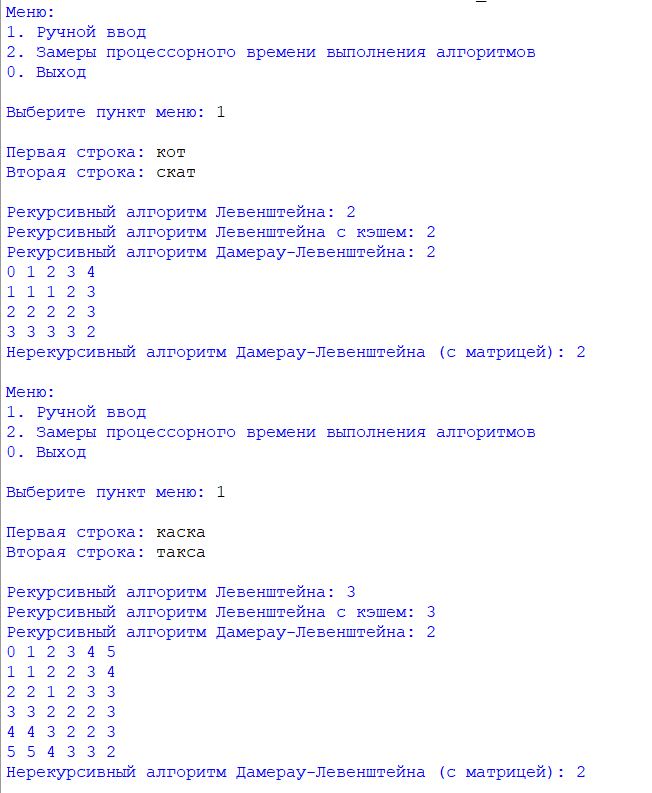
\includegraphics[scale=0.5]{example.png}
			\caption{Работа алгоритмов нахождения расстояния Левенштейна и Дамерау -- Левенштейна.}
		\end{center}
	\end{figure}
	
	\section{Технические характеристики}
	
	Ниже приведеные технические характеристики устройства, на котором было проведенно тестирование ПО:
	
	\begin{itemize}
		
		\item Операционная система: Windows 10 64-bit Home \cite{home}.
		
		\item Оперативная память: 8 GB.
		
		\item Процессор: 11th Gen Intel(R) Core(TM) i3-1115G4 @ 3.00GHz
		\cite{i3}.
		
	\end{itemize}
	
	\section{Время выполнения алгоритмов}
	Время выполнения алгоритмов замерялось с помощью функции process\_time модуля time в Python  \cite{process}. Данная функция возвращает значение в долях секунды суммы системного и пользовательского процессорного времени текущего процесса. \newline
	
	В таблице 4.1. представлены замеры времени работы для каждого из алгоритмов.
	
	\begin{table} [h!]
		\caption{Таблица времени выполнения алгоритмов (в долях секунды)}
		\begin{center}
			\begin{tabular}{|c c c c c|} 
				\hline
				Длина строк & RecLev & RecLevCache & RecDam & IterDam \\  
				\hline
				2 & 0.000000 & 0.000000 & 0.000000 & 0.000000\\
				\hline
				4 & 0.000156 & 0.000000 & 0.000156 & 0.000000\\
				\hline
				6 & 0.002812 & 0.000000 & 0.002812 & 0.000000 \\
				\hline
				8 & 0.086719 & 0.000000 & 0.078437 & 0.000000 \\
				\hline
				10 & 2.614063 & 0.000000 & 2.390938 & 0.000000\\
				\hline
				60 & NaN & 0.002812 & NaN & 0.001875\\
				\hline
				110 & NaN & 0.009375 & NaN & 0.006094\\
				\hline
				160 & NaN & 0.020000 & NaN & 0.012969\\
				\hline
				210 & NaN & 0.034531 & NaN & 0.021406\\
				\hline
				260 & NaN & 0.053125 & NaN & 0.033438\\
				\hline
				310 & NaN & 0.077188 & NaN & 0.048438\\
				\hline
				360 & NaN & 0.106875 & NaN & 0.067969\\
				\hline
				410 & NaN & 0.140469 & NaN & 0.089531\\
				\hline
				460 & NaN & 0.179375 & NaN & 0.115156\\
				\hline
			\end{tabular}
		\end{center}
	\end{table}
	
	\begin{figure}[h!]
		\begin{center}
			\begin{tikzpicture}
				\begin{axis}[
					legend pos = north west,
					xlabel=длина строки,
					ylabel=секунды,
					minor tick num = 1,
					grid = both,
					major grid style = {lightgray},
					minor grid style = {lightgray!25},
					xtick distance = 50,
					width = 0.9\textwidth,
					height = 0.5\textwidth]
					
					\addplot[
					blue,
					semithick,
					mark = x,
					mark size = 3pt,
					thick,
					] file {LevRec.txt};
					
					\addplot[
					red,
					semithick,
					mark = *,
					] file {LevCache.txt};
					
					\legend{
						Рекурсивный алгоритм Левенштейна,
						Рекурсивный алгоритм Левенштейна с кэшем
					}
				\end{axis}
			\end{tikzpicture}
		\end{center}
		\caption{Сравнение рекурсивного алгоритма Левенштейна и рекурсивного с кэшем}
	\end{figure}
	
	\begin{figure}[h!]
		\begin{center}
			\begin{tikzpicture}
				\begin{axis}[
					legend pos = north west,
					xlabel=длина строки,
					ylabel=секунды,
					minor tick num = 1,
					grid = both,
					major grid style = {lightgray},
					minor grid style = {lightgray!25},
					xtick distance = 50,
					width = 0.9\textwidth,
					height = 0.5\textwidth]
					
					\addplot[
					blue,
					semithick,
					mark = x,
					mark size = 3pt,
					thick,
					] file {LevRec.txt};
					
					\addplot[
					red,
					semithick,
					mark = *,
					] file {DamLevRec.txt};
					
					\legend{
						Расстояние Левенштейна,
						Расстояние Дамерау -- Левенштейна
					}
				\end{axis}
			\end{tikzpicture}
		\end{center}
		\caption{Сравнение рекурсивных алгоритмов нахождения расстояния Левенштейна и Дамерау-Левенштейна}
	\end{figure}
	
	\section{Использование памяти}
	
	Алгоритмы нахождения расстояния Левенштейна и Дамерау — Левенштейна не отличаются друг от друга с точки зрения использования памяти.
	
	Максимальная глубина стека вызовов при рекурсивной реализации равна сумме длин входящих строк. Поэтому, максимальный расход памяти равен: 
	
	\begin{equation}
		(\mathcal{S}(STR_1) + \mathcal{S}(STR_2)) \cdot (2 \cdot \mathcal{S}\mathrm{(string)} + 2 \cdot \mathcal{S}\mathrm{(integer)}),
	\end{equation}
	
	\noindent где $\mathcal{S}$ — оператор вычисления размера, $STR_1$, $STR_2$ — строки, $\mathrm{string}$ — строковый тип, 
	
	\noindent $\mathrm{integer}$ — целочисленный тип.
	
	Использование памяти при итеративной реализации теоретически равно:
	\begin{equation}
		(\mathcal{S}(STR_1) + 1) \cdot (\mathcal{S}(STR_2) + 1) \cdot \mathcal{S}\mathrm{(integer)} + 5\cdot \mathcal{S}\mathrm{(integer)} + 2 \cdot \mathcal{S}\mathrm{(string)}.
	\end{equation}
	
	
	\section{Вывод}
	
	Обычная рекурсивная реализация алгоритма нахождения расстояния Левенштейна работает дольше реализации с кэшем и итеративной реализации, время работы этой реализации увеличивается в геометрической прогрессии. Рекурсивный метод при этом использует больше памяти, чем итеративный.
	
	
	\chapter*{Заключение}
	\addcontentsline{toc}{chapter}{Заключение}
	
	В ходе проделанной работы был изучен метод динамического программирования на материале реализации алгоритмов нахождения расстояния Левенштейна и Дамерау-Левенштейна. Также были изучены алгоритмы поиска расстояния Левенштейна и Дамерау-Левенштейна нахождения расстояния между строками и получены практические навыки раелизации указанных алгоритмов в матричной и рекурсивных версиях, а так же в версиях с мемоизацией.
	
	Экспериментально было подтверждено различие во временной эффективности рекурсивной и нерекурсивной реализаций выбранного алгоритма определения расстояния между строками при помощи разработаного программного обеспечения на материале замеров процессорного времени выполнения реализации на варьирующихся длинах строк. Рекурсивная реализация алгоритма Левенштейна проигрывает нерекурсивной по времени исполнения в несколько десятков раз. Так же стоит отметить, что итеративный алгоритм Левештейна выполняется немного быстрее, чем итеративный алгоритм Дамерау - Левенштейна, но в целом алгоритмы выполняются за примерно одинаковое время.
	
	Теоретически было рассчитано использование памяти в каждой из реализаций алгоритмов нахождения расстояния Левенштейна и Дамерау - Левенштейна.
	
	\addcontentsline{toc}{chapter}{Список литературы}
	
	\bibliographystyle{utf8gost705u}  % стилевой файл для оформления по ГОСТу
	
	\bibliography{biblio}          % имя библиографической базы (bib-файла)
	
\end{document}
